	\documentclass[11pt]{article}
\usepackage{graphicx,amssymb,amsmath,amstext,hyperref,graphics,float,eurosym,geometry,lineno,changebar}
\hypersetup{
    colorlinks=true,        % false: boxed links; true: colored links
    linkcolor=black,         % color of internal links (change box color with linkbordercolor)    https://www.sharelatex.com/learn/Hyperlinks
    citecolor=black,        % color of links to bibliography
    filecolor=black,      % color of file links
    urlcolor=black           % color of external links
}
\topmargin -.5in
\textheight 9in
\oddsidemargin -.25in
\evensidemargin -.25in
\textwidth 7in

\begin{document}

% ========== Edit your name here
\author{}
\title{TISuMR device specifications}
\maketitle

%\medskip
\section{Scope of this document}
TISuMR is a collaboration project between University of Southampton, University of Groningen and Karlsruhe Institute of Technology. The aim of the project is to develop technologies for NMR (nuclear magnetic resonance) compatible microfluidic perfusion culture of PCLS (precision cut liver slices). Different device designs are currently in use at different sites to achieve this purpose. Although all these designs are made for specific requirements, some aspects of the designs are required to be the same to be recognized as a variant of the same principle design.

This document defines the specifications for a device design to be qualified as a TISuMR device. All the TISuMR personnel will follow these requirements for device design if the device is used for TISuMR research. Possible variations are also given to cater specific needs of experiments.

Changes to this document will be decided in the TISuMR meetings. The intended changes will be communicated to all the partners before the meeting to think upon. All the partners should agree for a change to be made final. This document will be available on \url{https://github.com/marcel-utz/tisumr-device} to obtain the latest version of the document. Marcel Utz will own the master copy and will be responsible to implement the changes. A drawing of the purposed device is shown in Fig.\ref{fig:tisumr-device}

\section{Required Specifications}
\begin{itemize}
\item \textbf{Culture chamber geometry:} The culture chamber is circular in shape with a diameter of 7$\pm$1 mm and a depth of 500$\pm$100 $\mu$m. The overall thickness of the device is less than 1 mm.
\item \textbf{Perfusion geometry:} The perfusion fluid flows around the PCLS. There can be more than one inlets and outlets. The inlet and outlet channels have cross sectional dimensions of 200$\pm$100$\times$200$\pm$100 $\mu$m$^2$. 
\item \textbf{Chip or device material:} Polycarbonate is used for the chip or device fabrication.
\item \textbf{Temperature:}. The PCLS culture is performed at 37$\pm$0.5$^{\circ}$.
\item \textbf{Gas composition:} Either carbogen (95 \% O$_2$ + 5 \% carbon dioxide) or a mixture (80 \% O$_2$+ 10 \% nitrogen +5 \% carbon dioxide) is used for the culture.
\item \textbf{Viability standards:} ATP/ protein (pmol/$\mu$g)  value for a slice is used as viability standard. Slices with   ATP/ protein (pmol/$\mu$g) value of 6 or more will be considered viable. The protocol to measure ATP/protein will be the same.
\item \textbf{Medium composition:} William E  with Glutamax + Glucose (1.375 g/500mL William E medium) + Gentamycine (500$\mu$L/500mL)
\item \textbf{Sterilization:} Ethanol will be used for sterilization.
\end{itemize}

\section{Allowed variations}
\begin{itemize}
\item \textbf{Detailed fluidic paths:} Fluidic network can be designed freely.
\item \textbf{Flow protocol:} The media can be flowed by different types of pumps or centrifuge. 
\item \textbf{Fabrication method:} The devices can be made through machining or bonding layers by different protocols.
\item \textbf{Flow rates:}. Range of flow rates will be decided through optimization.
\end{itemize}

\begin{figure}
\centering
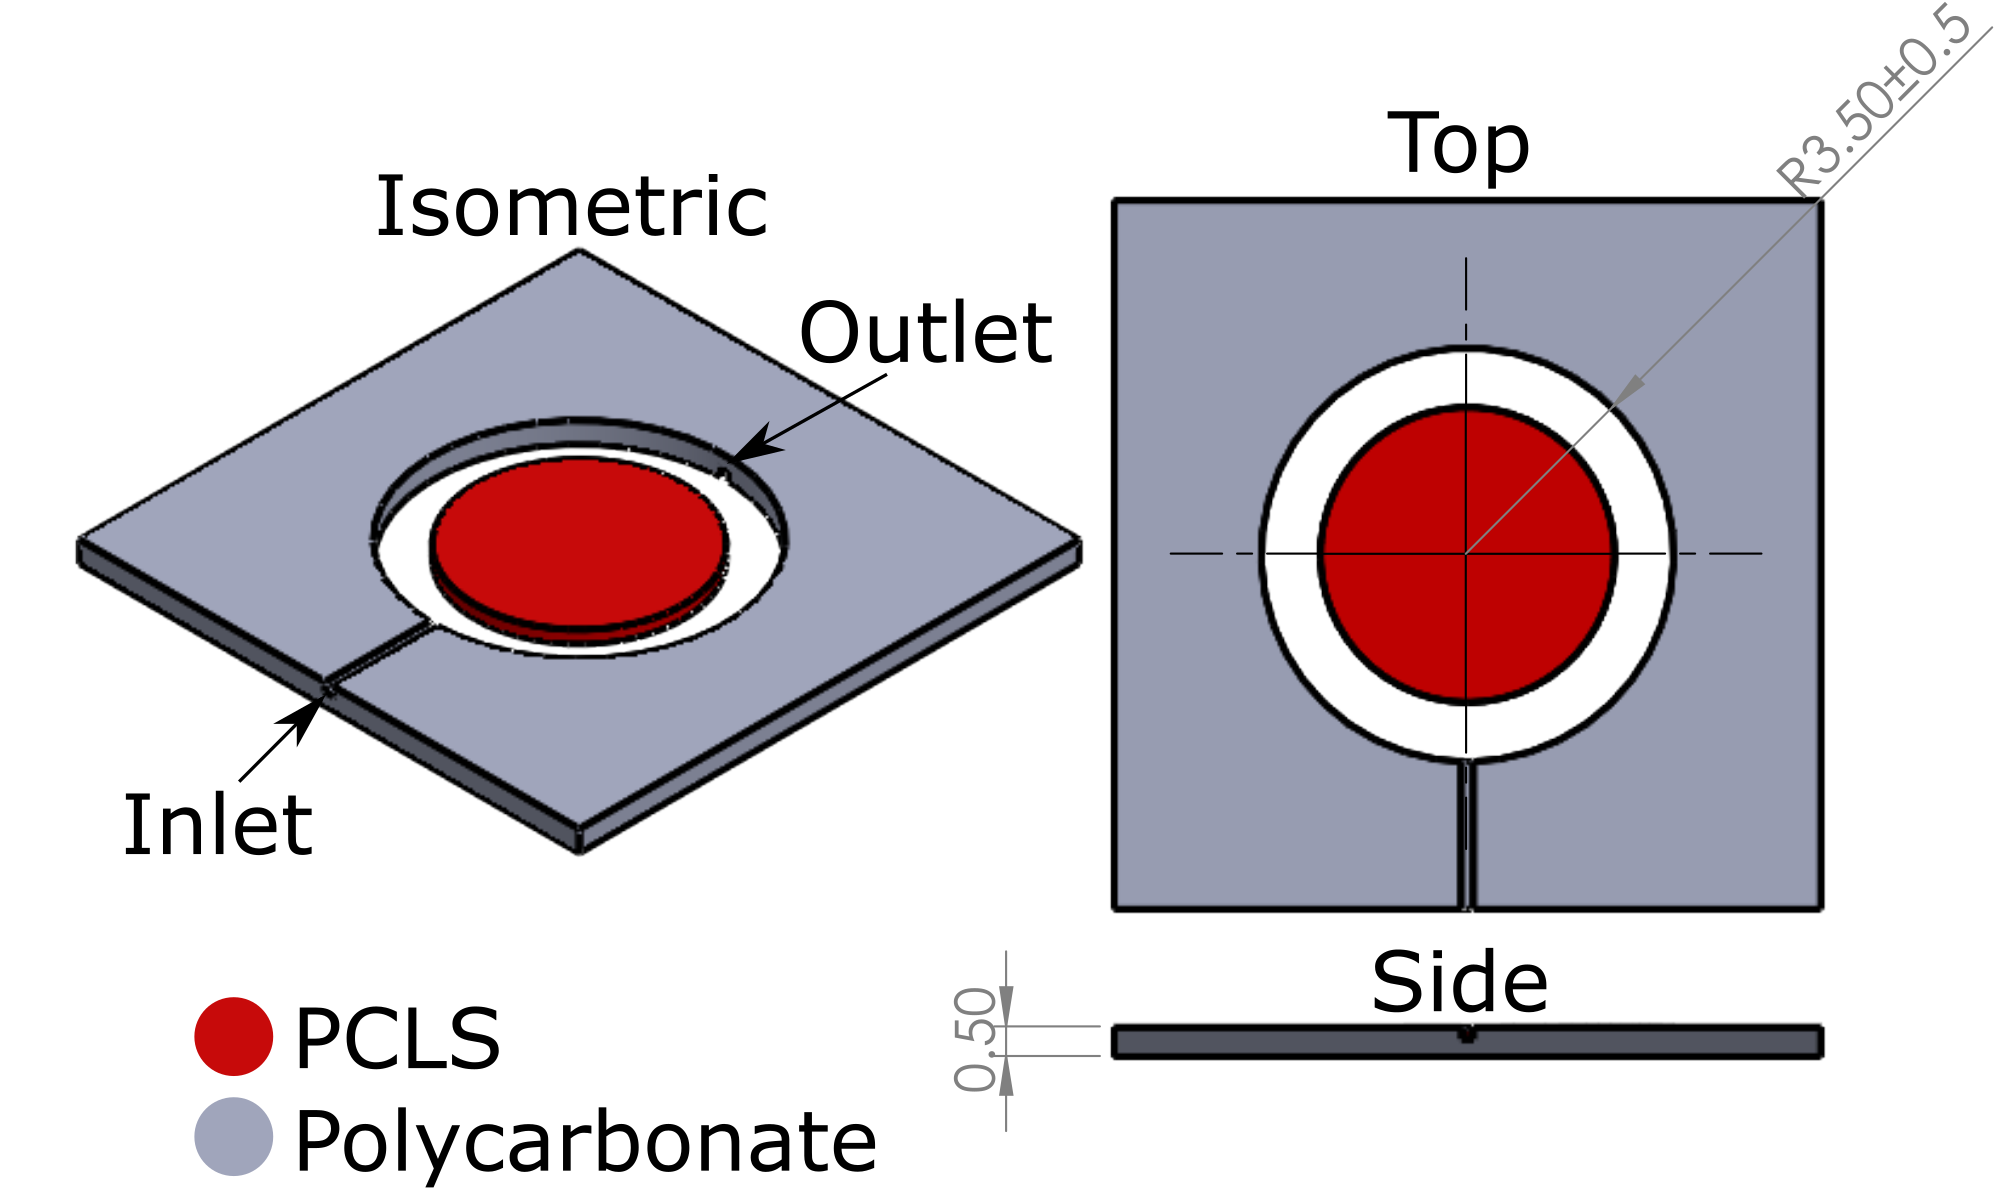
\includegraphics[width=.8\linewidth,keepaspectratio=true]{./device/tisumr-device.png}
\caption{Isometric, top and side views of the device. The diameter of the PCLS chamber is 0.7 mm. The thickness of the chamber is 0.5 mm.}
\label{fig:tisumr-device}
\end{figure}

\end{document}